% !TEX program = xelatex
\documentclass[10pt,aspectratio=43,mathserif]{beamer}		
%设置为 Beamer 文档类型,设置字体为 10pt,长宽比为16:9,数学字体为 serif 风格

%%%%-----导入宏包-----%%%%
\usepackage{seu}
\usepackage{xeCJK}
\usepackage{amsmath,amsfonts,amssymb,bm}
\usepackage{color}
\usepackage{graphicx,hyperref,url}
\usepackage{subfigure}	
%%%%%%%%%%%%%%%%%%


%%%%-----设置字体-----%%%%
%Windows和Mac OS下都可用
\setsansfont{Helvetica}

%\setsansfont{Times New Roman}

%仅Windows可用
%\setCJKmainfont{Hiragino Sans GB W3}

%仅Mac OS下可用
%\setCJKmainfont{Songti SC}




%设置 Beamer 主题
\beamertemplateballitem


\AtBeginSection[]
{
  \begin{frame}<beamer>
    \frametitle{\textbf{目录}}
    \textbf{\tableofcontents[currentsection]}
  \end{frame}
}


%%%%----首页信息设置----%%%%
\title[RF-based Blood Donor Recruitment]{\fontsize{13pt}{18pt}\selectfont {基于随机森林的献血招募模型}}
%\subtitle{\fontsize{9pt}{14pt}\selectfont \textbf{基于随机森林的献血招募模型}}			
%%%%----标题设置


\author[Zixing Song]{
  宋子星 \\
  %{\small {songzixing@seu.edu}
  }

%%%%----个人信息设置

\institute[SEU]{
  东南大学计算机科学与工程学院\\
  }
%%%%----机构信息

\date[\today]{
 \today}
%%%%----日期信息


\begin{document}

\begin{frame}
\titlepage
\end{frame}				%生成标题页



\section*{目录}

		\begin{frame}
		\frametitle{\textbf{目录}}
		\textbf{\tableofcontents}
		\end{frame}				%生成提纲页

\section{背景}

		\begin{frame}
            \frametitle{\textbf{背景}}

            \begin{block}{\textbf{现状与意义}}
                \begin{itemize}
                    \item 医疗领域:当前献血招募主要采取人力招募方式
                    \item 计算机领域:机器学习技术迅猛发展
                    \item 献血招募 + 机器学习 $\Rightarrow$ 提升招募精度 + 降低招募成本 ?
                \end{itemize}
            \end{block}

            \begin{figure}[!t]
                \centering 
                \subfigure{
                    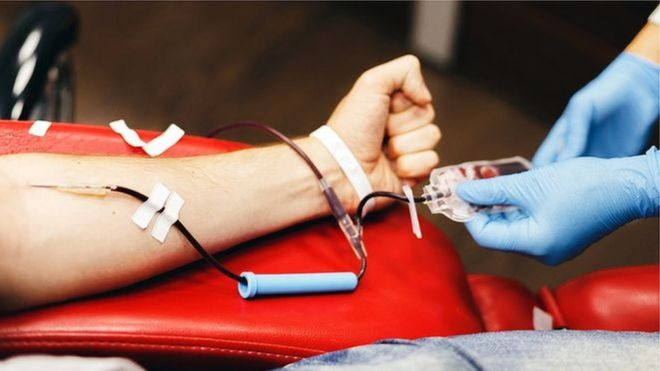
\includegraphics[width=2in]{figures/blood_donation.jpg}
                }
                \subfigure{
                    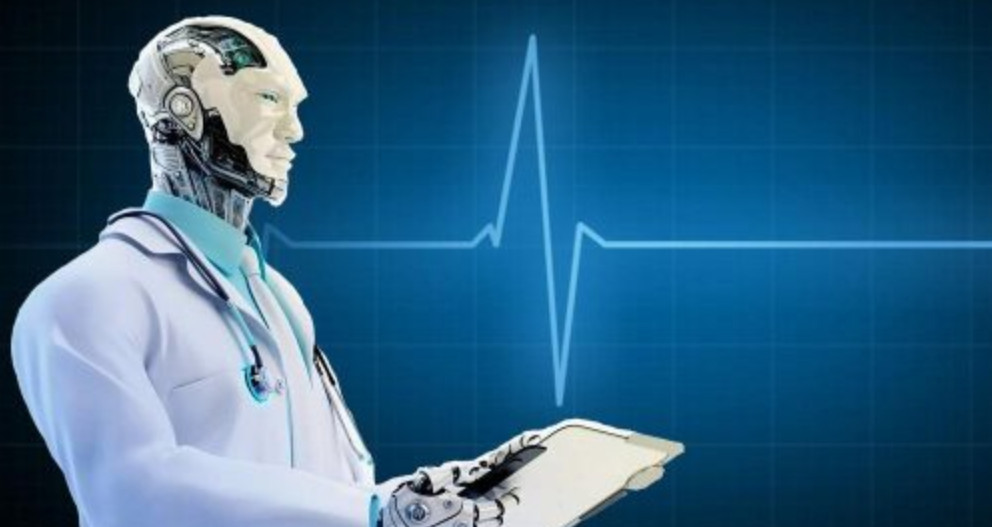
\includegraphics[width=2in]{figures/medical_AI.jpg}
                }
            \end{figure}

    \end{frame}

    \begin{frame}
        \frametitle{\textbf{研究问题}}
        \begin{figure}[!t]
            \centering 
            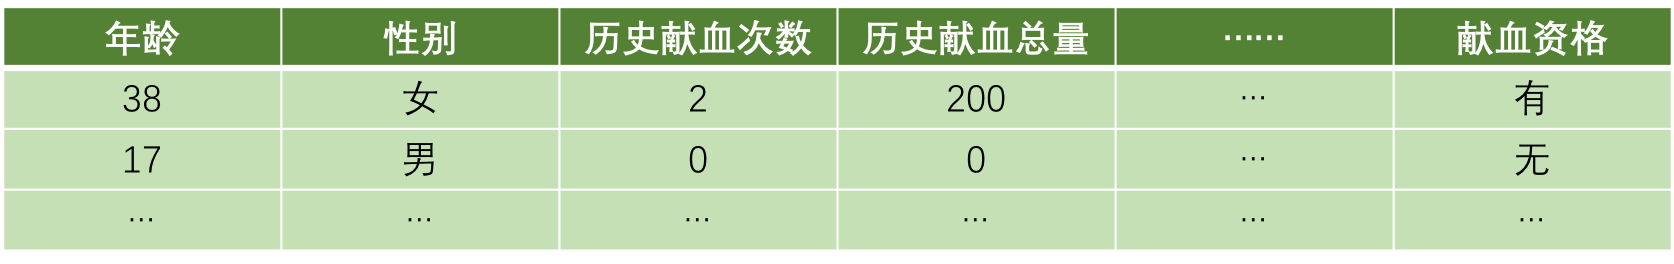
\includegraphics[width=4in]{figures/samples.png}
        \end{figure}
        
        \begin{figure}[!t]
            \centering 
            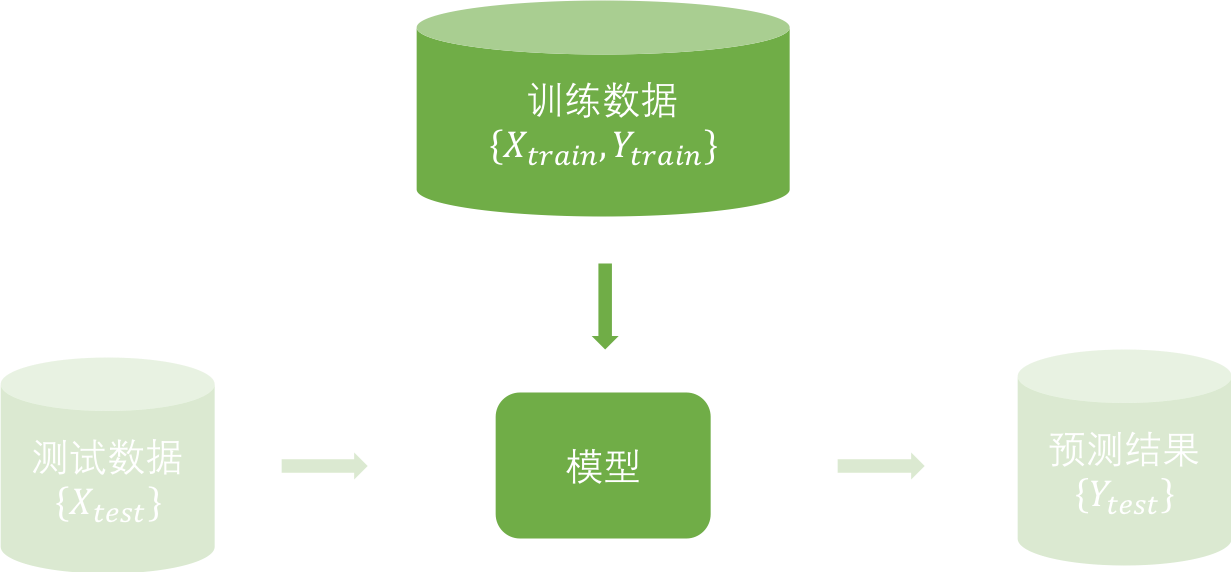
\includegraphics[width=4in]{figures/training1.png}
        \end{figure}

    \end{frame}

    \begin{frame}
        \frametitle{\textbf{研究问题}}
        \begin{figure}[!t]
            \centering 
            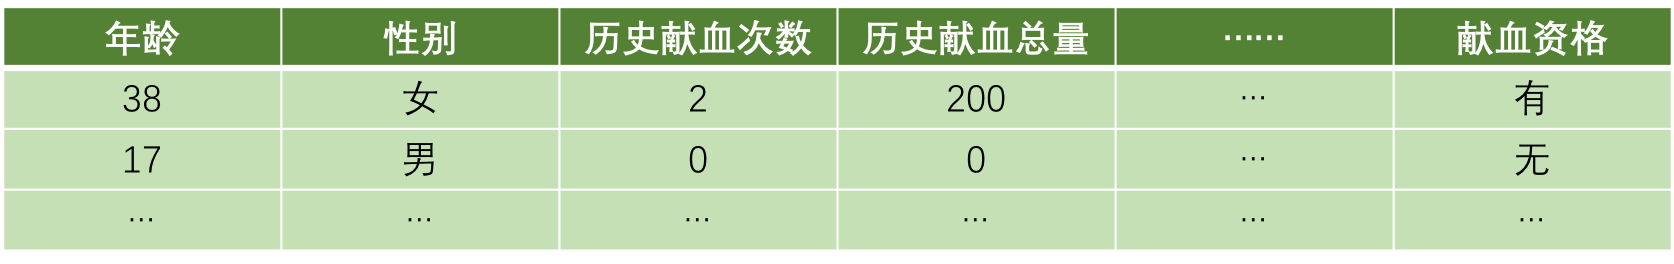
\includegraphics[width=4in]{figures/samples.png}
        \end{figure}
        
        \begin{figure}[!t]
            \centering 
            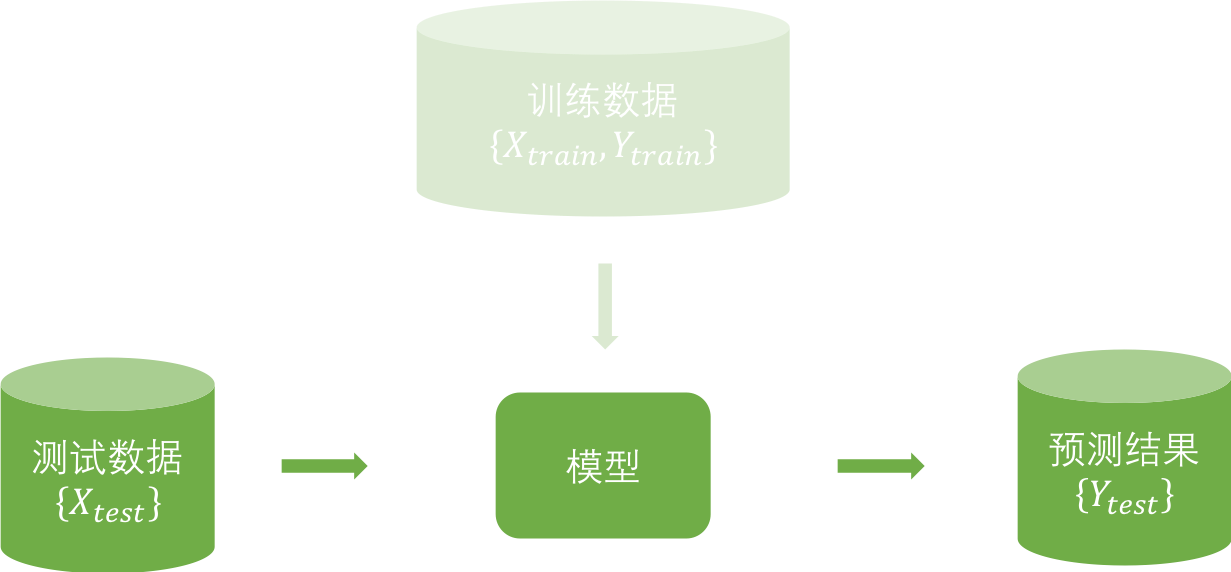
\includegraphics[width=4in]{figures/testing1.png}
        \end{figure}

    \end{frame}

\section[理论]{随机森林理论}

		\begin{frame}
		  \frametitle{\textbf{集成学习(Ensemble Learning)}}
            \begin{figure}[!t]
            \centering
            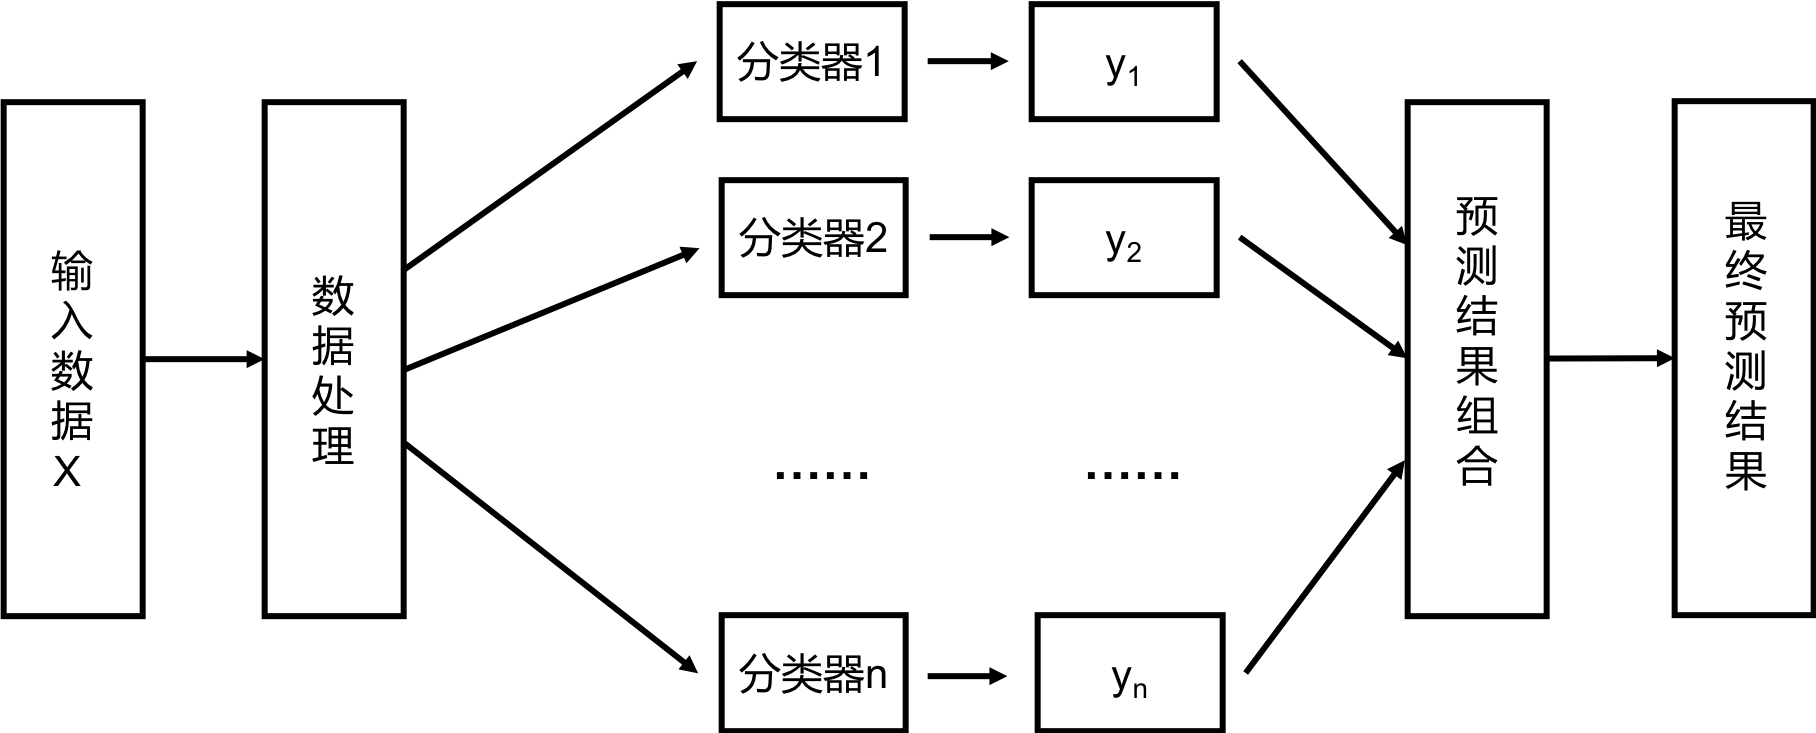
\includegraphics[width=4in]{figures/el.png}
            \caption{集成学习流程框架}
            \label{el}
            \end{figure}
            \textbf{集成学习}是指用于训练多个学习器并组合其输出,可以将其视为“决策委员会”的投票决策结果。
		\end{frame}

		\begin{frame}
		  \frametitle{\textbf{Bagging}}
            \begin{figure}[!t]
            \centering
            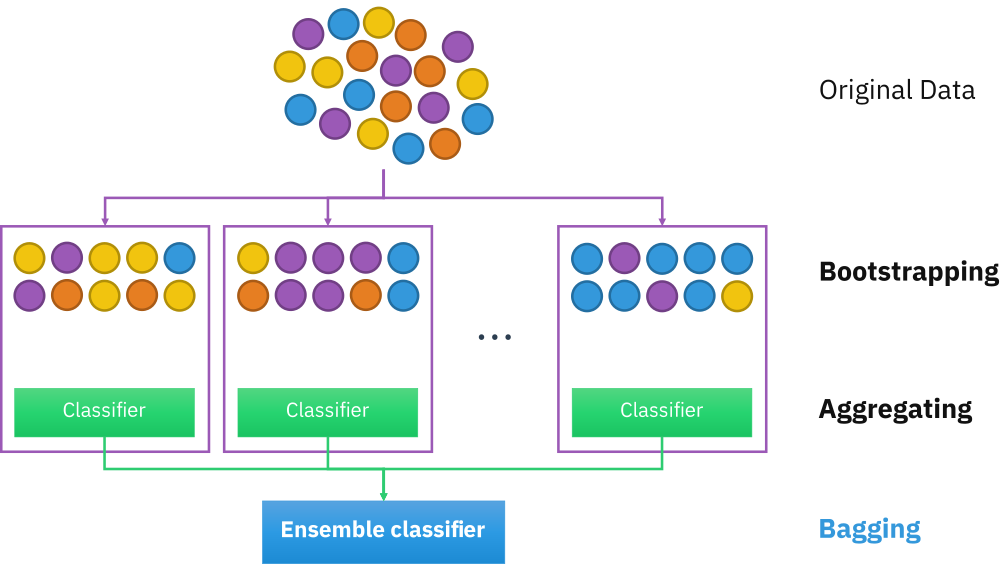
\includegraphics[width=3.5in]{figures/bagging.png}
            \caption{Bagging算法}
            \label{bagging}
            \end{figure}
            \textbf{Bagging}利用\textit{有放回抽样}生成新的训练数据集(Bootstrap samples)。
		\end{frame}

        \begin{frame}
		  \frametitle{\textbf{决策树 (Desicion Tree)}}
            \begin{columns}
                \column{.5\textwidth}
                \footnotesize
                \begin{figure}[!t]
                    \centering
                    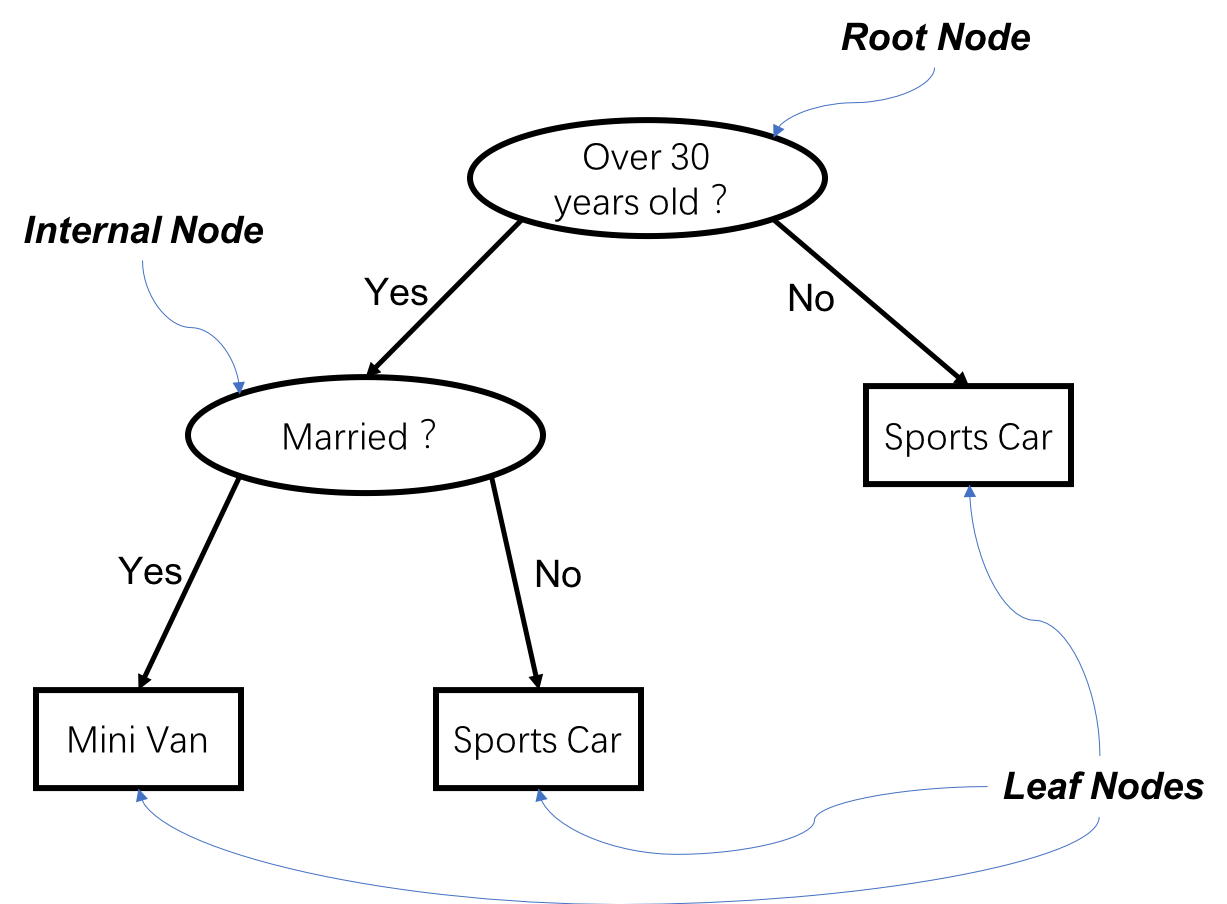
\includegraphics[width=1.1\textwidth]{figures/dt_eg.png}
                    \caption{决策树案例}
                    \label{figure3_OTT}
                \end{figure}

                \column{.5\textwidth}
                \begin{figure}[!t]
                    \centering
                    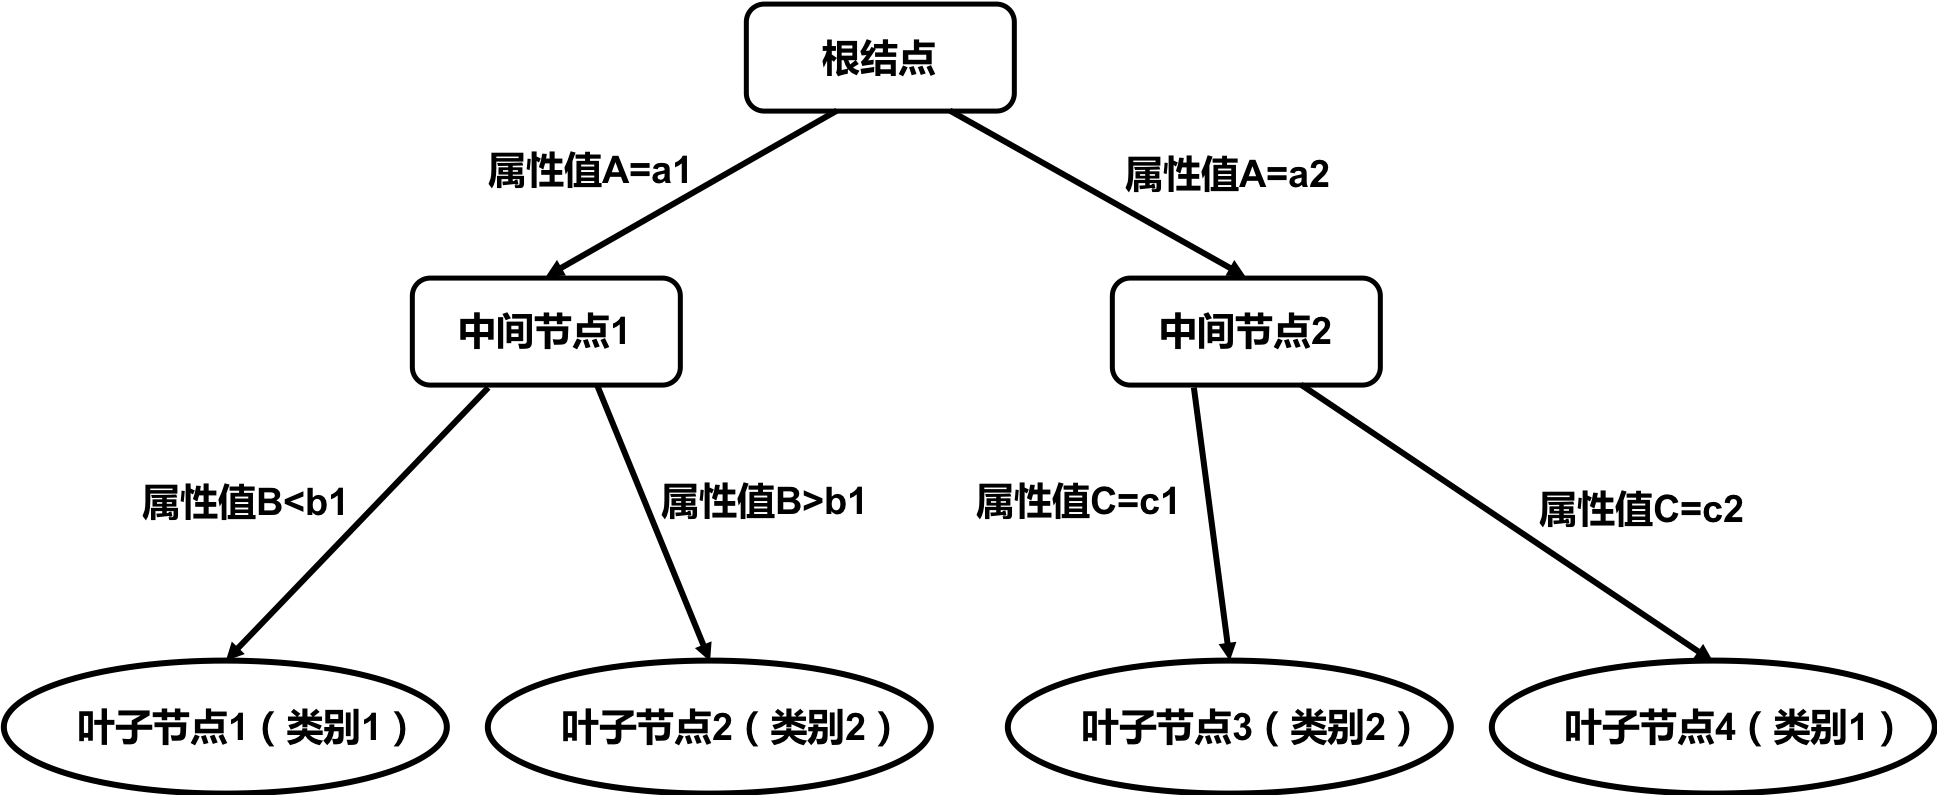
\includegraphics[width=1.1\textwidth]{figures/dt_general.png}
                    \caption{决策树归纳案例}
                    \label{figure3_OTT}
                \end{figure}
            \end{columns}
            决策树的训练:构建一棵决策树(ID3,C4.5,CART)。\\
            决策树的测试:自顶而下匹配一条路径。
        \end{frame}
        
        \begin{frame}
            \frametitle{\textbf{决策树生成算法}}
            \begin{columns}
                \column{.4\textwidth}
                \footnotesize
                \begin{itemize}
                    \item 训练集样本特征:性别、年龄和职业。
                    \item 预测目标:是否喜欢玩电脑游戏。
                    \item 算法关键:每次寻找出当前最佳分割属性。
                \end{itemize}

                \column{.6\textwidth}
                \begin{figure}[!t]
                    \centering
                    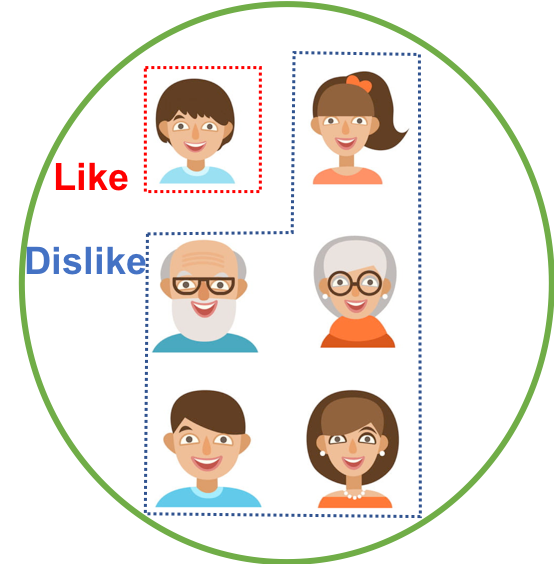
\includegraphics[width=1\textwidth]{figures/dt_gen_0.png}
                \end{figure}
            \end{columns}
        \end{frame}

        \begin{frame}
            \frametitle{\textbf{决策树生成算法}}
            \begin{columns}
                \column{.4\textwidth}
                \footnotesize
                \begin{itemize}
                    \item 训练集样本特征:性别、年龄和职业。
                    \item 预测目标:是否喜欢玩电脑游戏。
                    \item 根据某分割指标,从3个属性中选择\textbf{年龄}作为分割属性,分裂节点。
                    \item 无需分割,则停止分裂节点。
                \end{itemize}

                \column{.6\textwidth}
                \begin{figure}[!t]
                    \centering
                    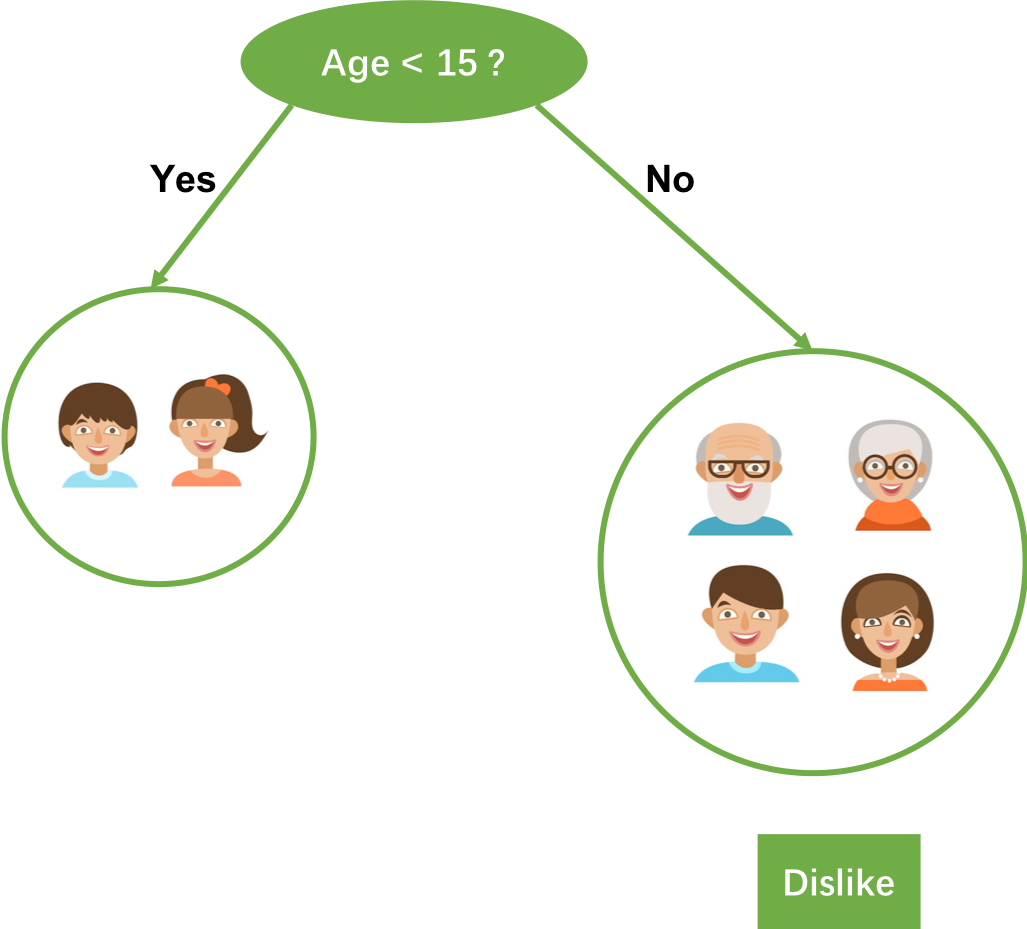
\includegraphics[width=1.1\textwidth]{figures/dt_gen_1.png}
                \end{figure}
            \end{columns}
        \end{frame}

        \begin{frame}
            \frametitle{\textbf{决策树生成算法}}
            \begin{columns}
                \column{.4\textwidth}
                \footnotesize
                \begin{itemize}
                    \item 训练集样本特征:性别、年龄和职业。
                    \item 预测目标:是否喜欢玩电脑游戏。
                    \item 对需要再次分割的节点,根据某分割指标,从剩下的2个属性中选择\textbf{性别}作为分割属性,分裂节点。
                \end{itemize}

                \column{.6\textwidth}
                \begin{figure}[!t]
                    \centering
                    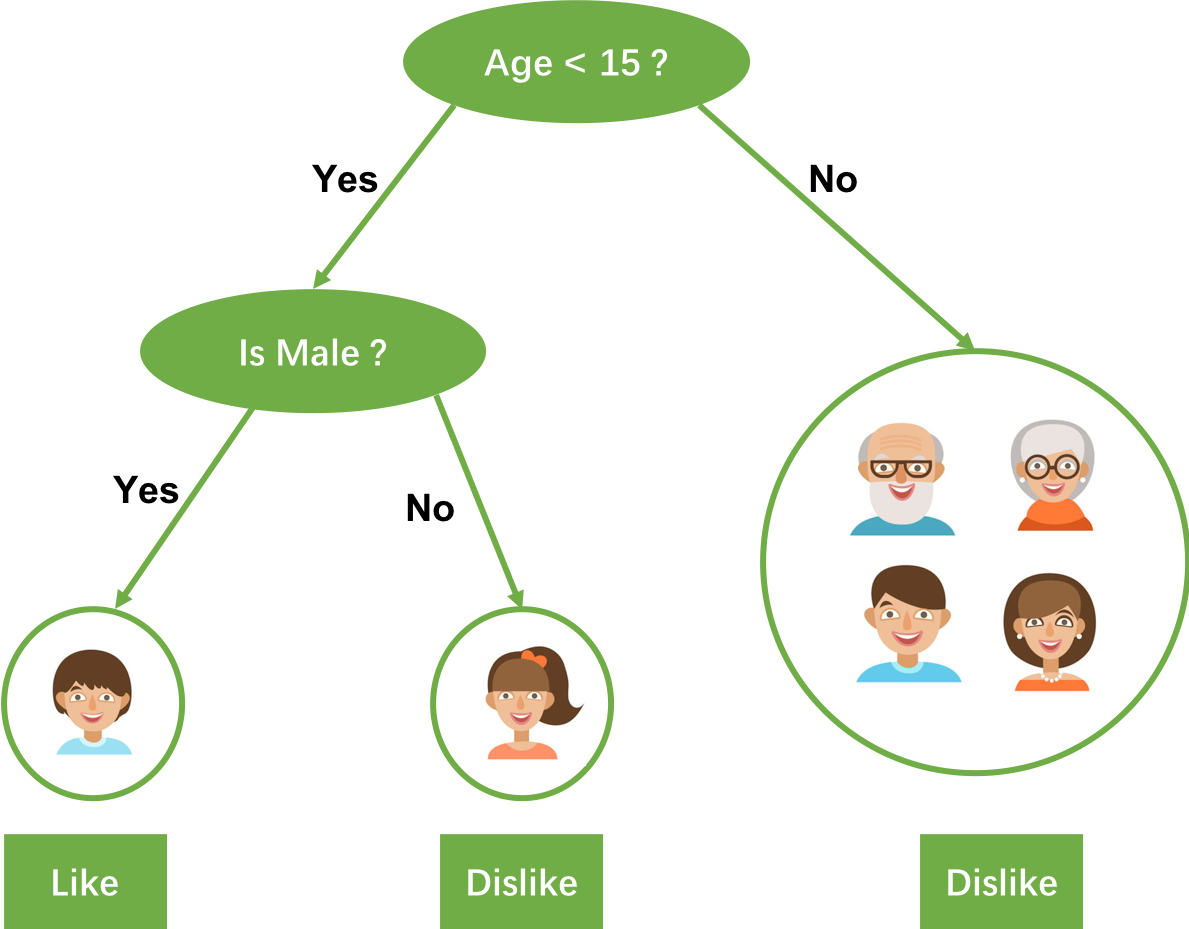
\includegraphics[width=1.1\textwidth]{figures/dt_gen.png}
                \end{figure}
            \end{columns}
        \end{frame}

        \begin{frame}
            \frametitle{\textbf{决策树生成算法}}
            \begin{table}[htbp!]
                \caption{三种最常见的决策树生成算法比较}
                \label{dt_compare}
                \centering
                \begin{tabular}{c c c c c c}
                \hline
                生成算法 & 分割指标  & 支持的属性 & 缺失值处理 \\ \hline
                ID3 & 信息增益 & 仅离散属性 & 不支持\\     
                C4.5 & 信息增益率  & 离散、连续属性 & 支持\\    
                CART & 基尼指数 & 离散、连续属性 & 支持 \\ \hline
                \end{tabular}
            \end{table}
        \end{frame}

        \begin{frame}
            \frametitle{\textbf{随机森林 (Random Forest)}}
            \begin{block}{\textbf{随机森林的随机性}}
                \begin{itemize}
                  \item 随机森林 = Bagging + 决策树(CART)
                  \item 训练集生成的随机性 $\Rightarrow$ Bagging (Bootstrap样本)
                  \item 特征变量选取的随机性 $\Rightarrow$ 决策树生成中,每次分裂节点时,随机选择一部分特征作为候选分割属性,
                    常见$M=\sqrt{N}$,$M=\log _2{N}$,再从候选属性中,寻找出最佳分割属性。
                \end{itemize}
            \end{block}
        \end{frame}

        \begin{frame}
            \frametitle{\textbf{随机森林 (Random Forest)}}
              \begin{columns}
                  \column{.5\textwidth}
                  \footnotesize
                  \begin{figure}[!t]
                      \centering
                      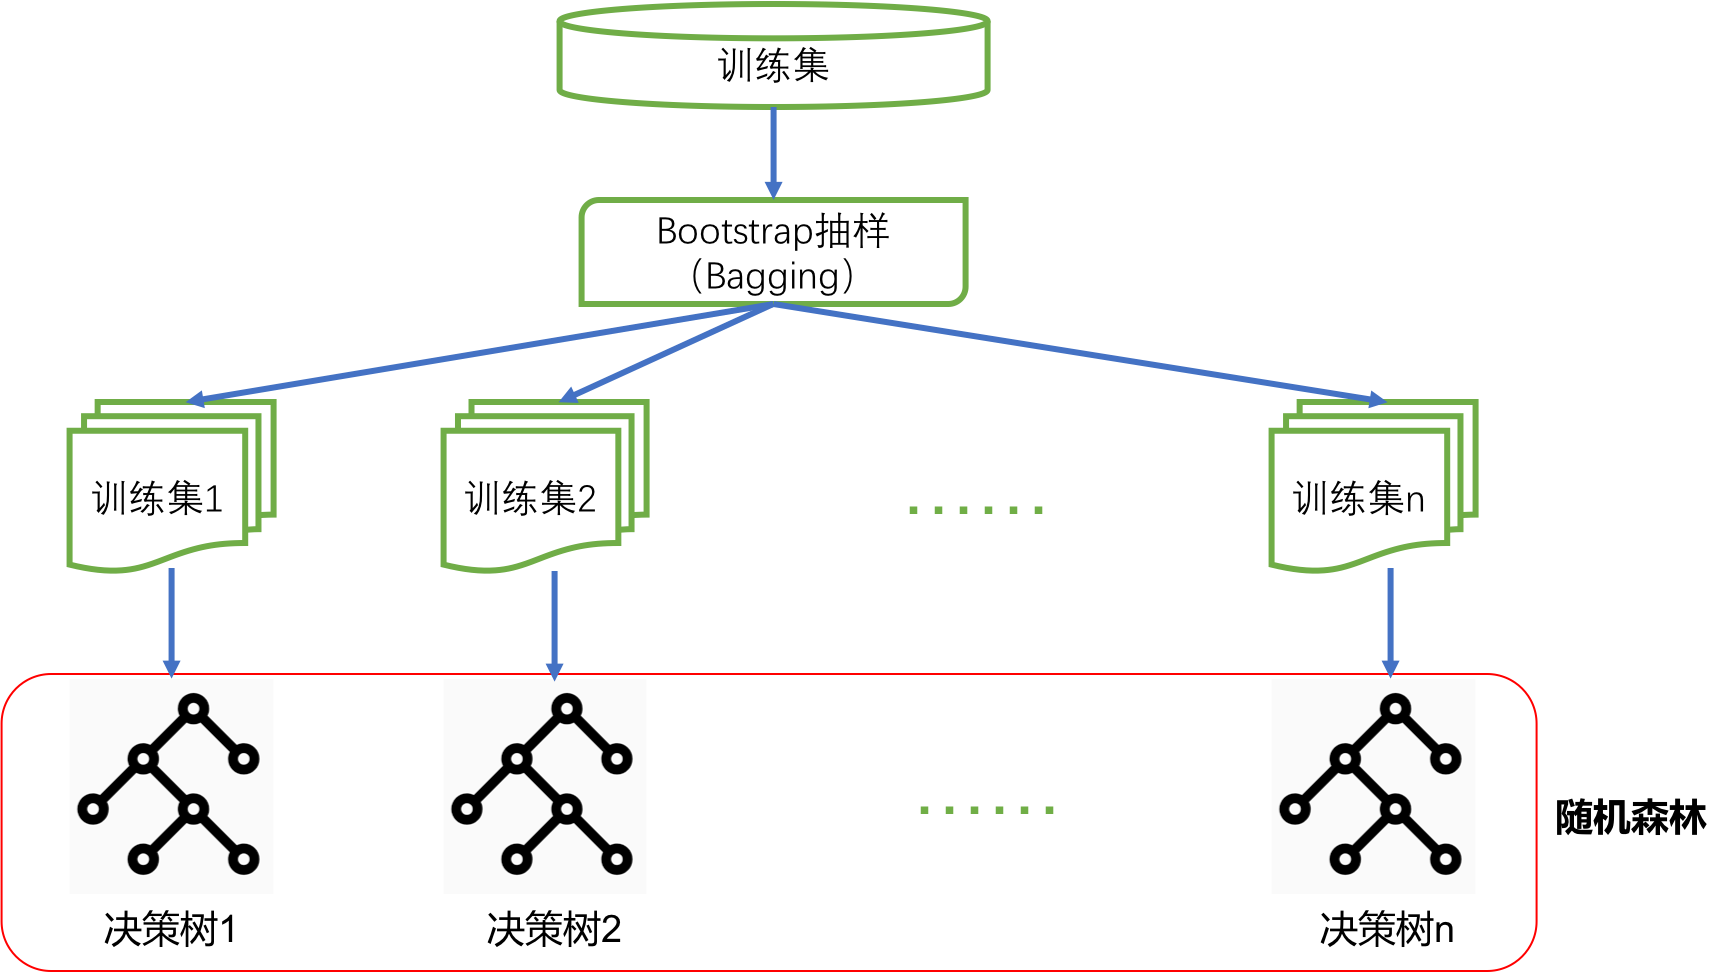
\includegraphics[width=1.15\textwidth]{figures/rf_training.png}
                      \caption{随机森林训练过程}
                  \end{figure}
  
                  \column{.5\textwidth}
                  \begin{figure}[!t]
                      \centering
                      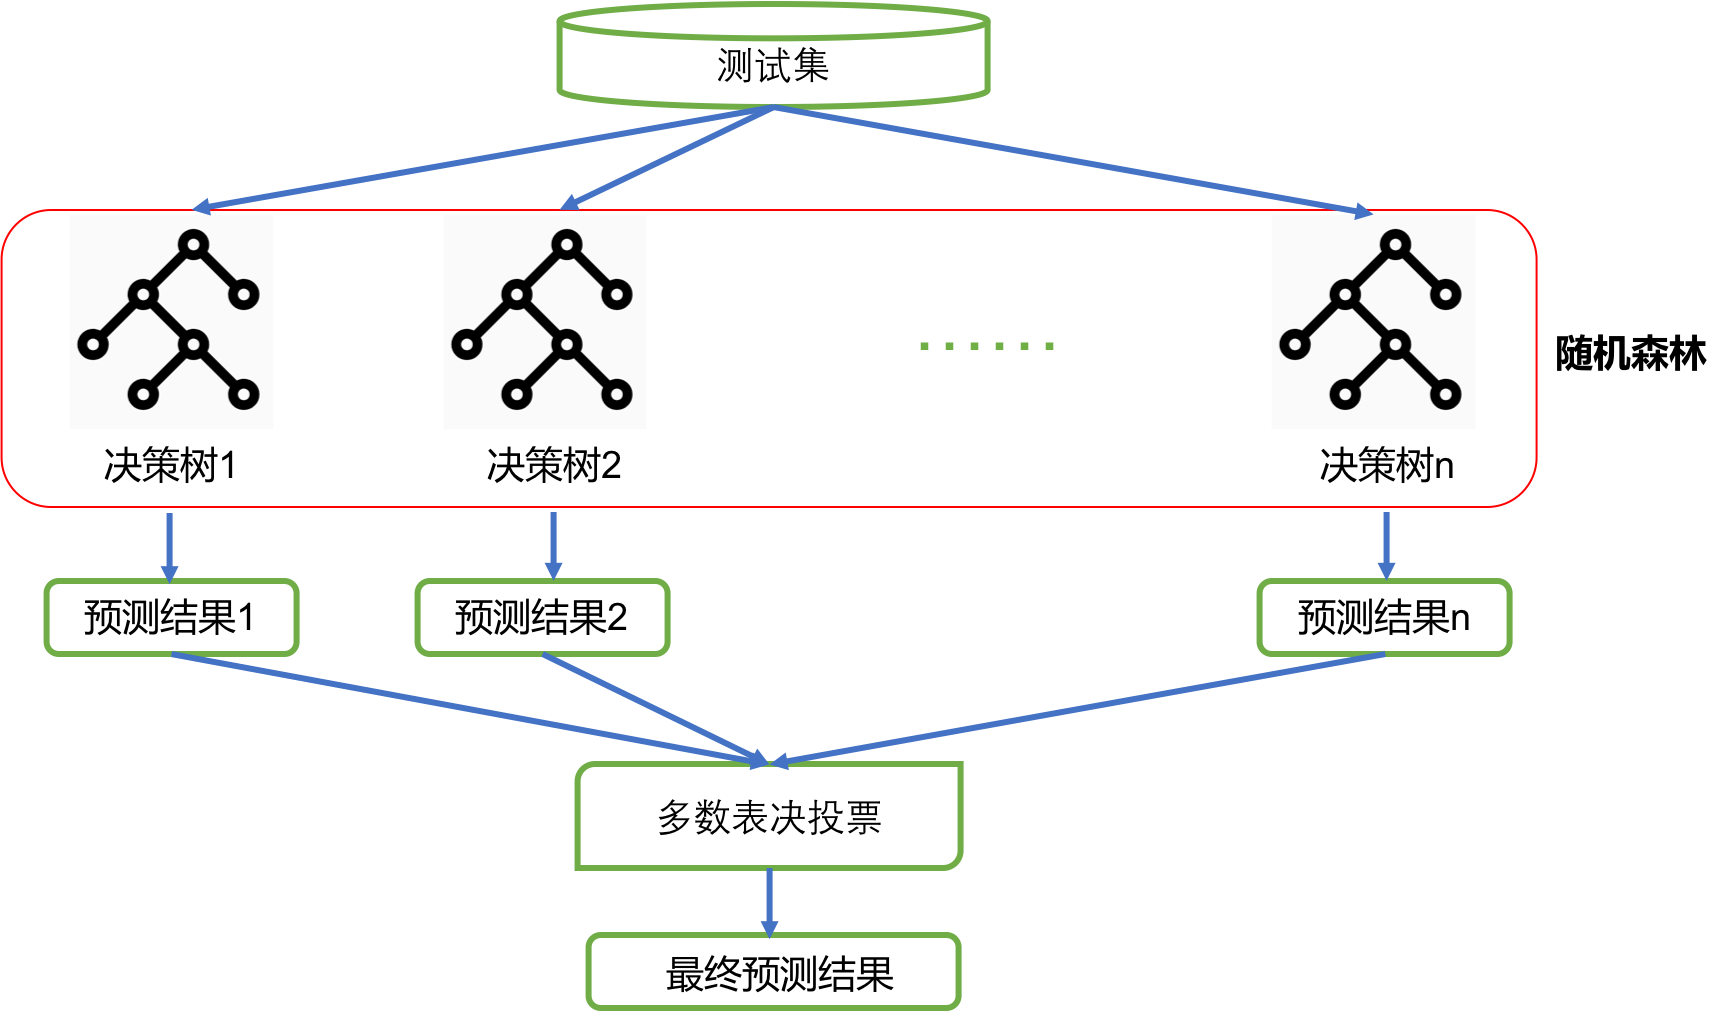
\includegraphics[width=1.1\textwidth]{figures/rf_testing.png}
                      \caption{随机森林测试过程}
                  \end{figure}
              \end{columns}
          \end{frame}

\section[方法]{研究方法与数据集特征}


		\begin{frame}
		  \frametitle{\textbf{爬取公共短消息网关}}
            % ----------------分栏的结构开始---------------- %
            % 该结构中使用block分开两个内容区
            % 可根据需要进行图文混排?我还没试过,我想应该可以
            \begin{columns}
                \column{.5\textwidth}
                \footnotesize
                \begin{itemize}
                  \item 使用Scrapy框架爬取公共网关
                  \item 收集8个公共短信网关在14个月的数据
                  \item 共抓取386,327条数据
                \end{itemize}

                \column{.5\textwidth}
                \begin{table}
                \caption{公共网关及抓取的信息数}
                \label{table1:gateways}
                \centering
                \footnotesize
                \begin{tabular}{|c|c|}
                \hline
                \textbf{Site}           & \textbf{Messages}\\
                \hline
                receivesmsonline.net    &81313\\
                \hline
                receive-sms-online.info &69389\\
                \hline
                receive-sms-now.com     &63797\\
                \hline
                 hs3x.com               &55499\\
                \hline
                receivesmsonline.com    &44640\\
                \hline
                receivefreesms.com      &37485\\
                \hline
                receive-sms-online.com  &27094\\
                \hline
                 e-receivesms.com       &7107\\
                \hline
                \end{tabular}
                \end{table}
            \end{columns}

		\end{frame}

        \begin{frame}
		  \frametitle{\textbf{消息聚类分析}}
            \begin{block}{\textbf{基本思路}}
                \begin{itemize}
                    \item 使用编辑距离矩阵将类似的消息归于一张连通图中。
                    \item 使用固定值替换感兴趣的消息,如代码、email地址。
                    \item 查找归一化距离小于阈值的消息,并确定聚类边界。
                \end{itemize}
            \end{block}

            \begin{block}{\textbf{实现步骤}}
                \begin{enumerate}
                  \item 加载所有消息。
                  \item 用固定的字符串替换数字、电子邮件和URL以预处理消息。
                  \item 将预处理后的信息按字母排序。
                  \item 通过使用编辑距离阈值(0.9)来确定聚类边界。
                  \item 手动标记各个聚类,以确定服务提供者、消息类别等。
                \end{enumerate}
            \end{block}
		\end{frame}

        \begin{frame}
		  \frametitle{\textbf{消息分类结果}}
            \begin{itemize}
                \item \textbf{账户创建确认信息}:向来自服务提供者的用户提供了一个代码,该服务提供者需要在新帐户创建期间进行SMS验证。
                \item \textbf{活动确认信息}:向来自服务提供者的用户提供了请求授权进行活动的代码(例如,付款确认)。
                \item \textbf{一次性密码}:包含用户登录的代码的短信息。
                \item \textbf{用于绑定不同设备的一次性口令}:将消息发送给用户,以绑定一个新的电话号码或启用相应的移动应用程序。
                \item \textbf{重置密码口令}:包含密码重置密码的短信息。
                \item \textbf{其他}:其他未被指定为某种特定功能的消息。
            \end{itemize}
		\end{frame}

        \begin{frame}
		  \frametitle{\textbf{消息分类结果}}
            \begin{columns}
                \column{.5\textwidth}
                \footnotesize
                \begin{itemize}
                  \item 账户创建和移动设备绑定占比最大,占51.6\%
                  \item 一次性密码信息占7.6\%
                  \item 密码重置消息占1.3\%
                  \item 包含“测试”关键词的消息占0.8\%
                \end{itemize}

                \column{.5\textwidth}
                \begin{figure}[!t]
                    \centering
                    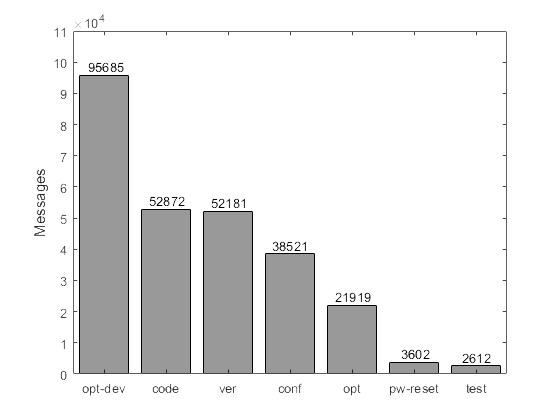
\includegraphics[width=1.1\textwidth]{figures/figure4.png}
                    \caption{消息的聚类}
                    \label{figure3_OTT}
                \end{figure}
            \end{columns}
		\end{frame}



\section[分析]{SMS使用情况分析}


		\begin{frame}
		  \frametitle{\textbf{使用SMS作为安全信道}}
		  \begin{block}{\textbf{PII和其他敏感信息}}
                \begin{itemize}
                    \item 财务信息
                    \item 用户名和密码
                    \item 重置密码口令
                    \item 其他个人识别信息(PII)
                    \item 敏感程序的SMS活动
                \end{itemize}
            \end{block}
		\end{frame}

        \begin{frame}
		  \frametitle{\textbf{使用SMS作为安全信道}}
            \begin{block}{\textbf{SMS编码熵}}
                使用 $\chi$方检验测试每组编码的熵。$\chi$方检验是一个零假设的显著性检验,用于测试SMS服务的编码是否是从低位到高位均匀分布的。若p值小于0.01,则表明观测值和理想均匀分布之间存在统计学上的显著差异。
                检验结果表明,65\%的SMS服务的编码熵较低,容易被预测和攻击。
            \end{block}
            \begin{columns}

                \column{.26\textwidth}
                \begin{figure}
                    \centering
                    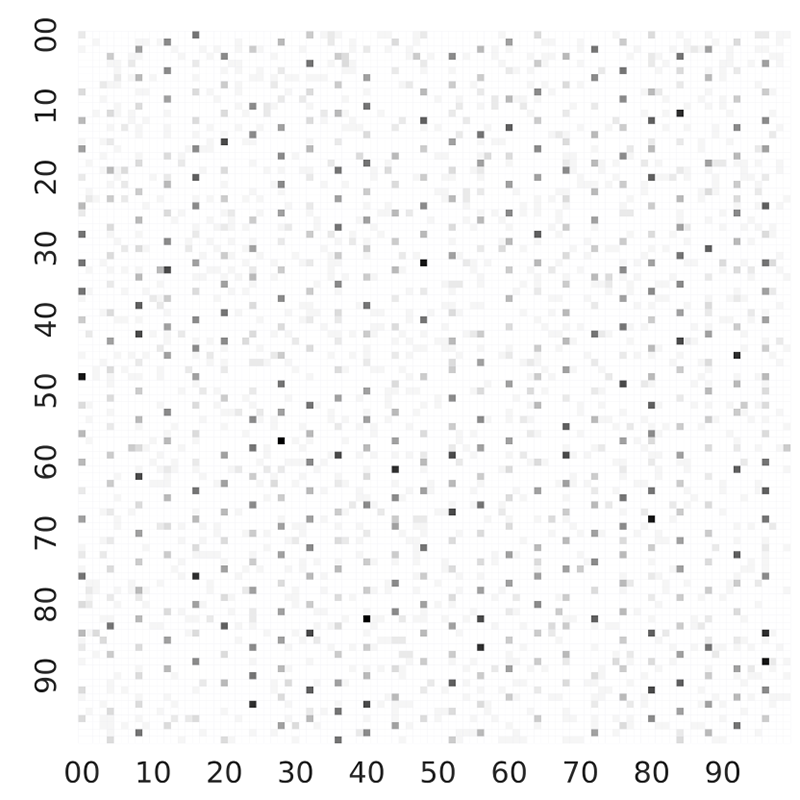
\includegraphics[width=1.1\textwidth]{figures/figure6.png}
                    \caption{WeChat}
                    \label{figure6_WeChat}
                \end{figure}

                \column{.26\textwidth}
                \begin{figure}
                    \centering
                    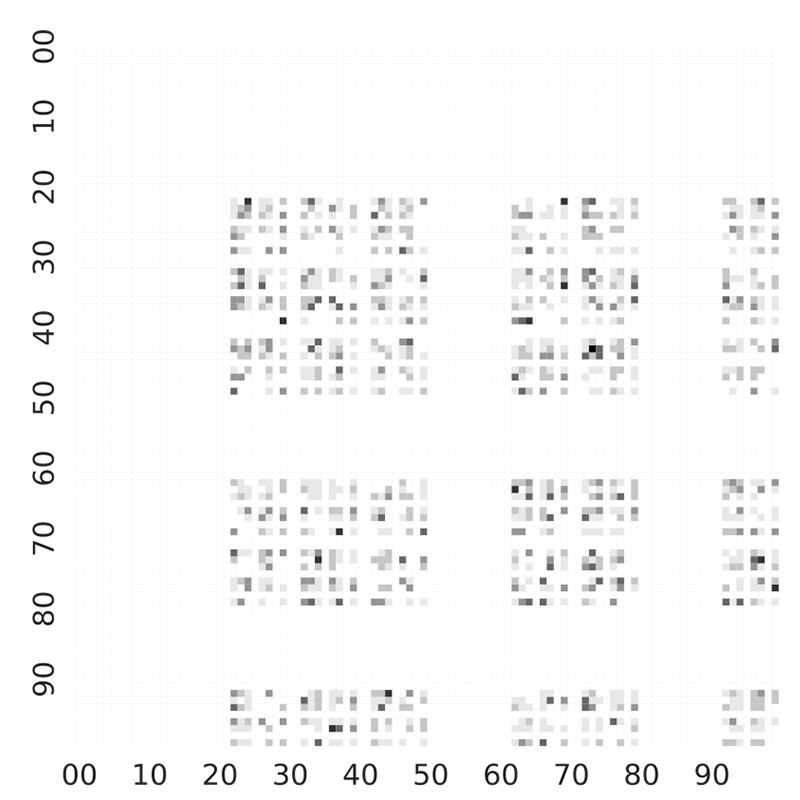
\includegraphics[width=1.1\textwidth]{figures/figure7.png}
                    \caption{Talk2}
                    \label{figure3_Talk2}
                \end{figure}

                \column{.26\textwidth}
                \begin{figure}
                    \centering
                    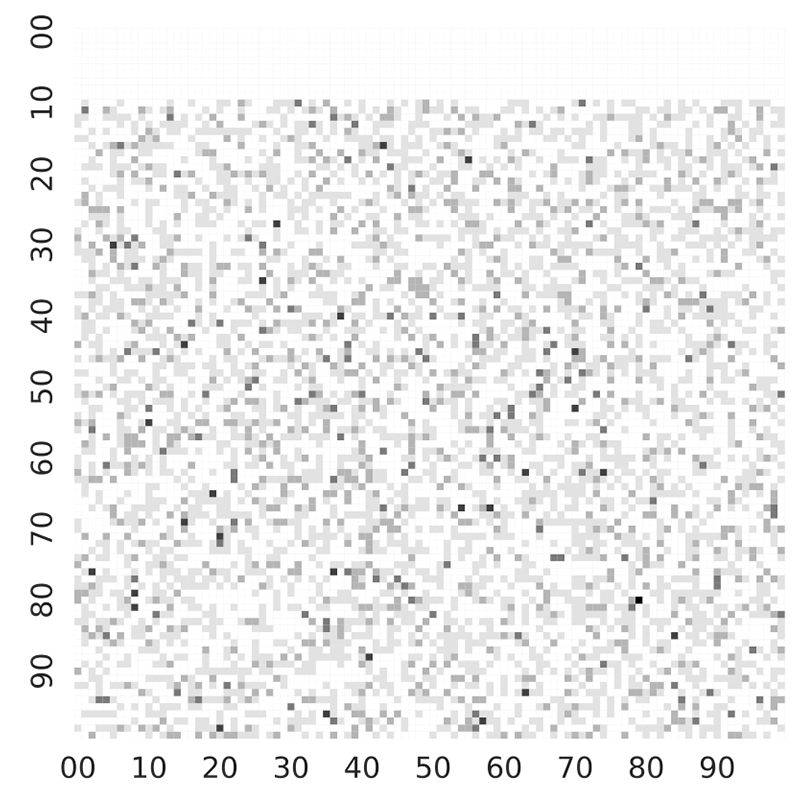
\includegraphics[width=1.1\textwidth]{figures/figure8.png}
                    \caption{Google}
                    \label{figure3_Google}
                \end{figure}

            \end{columns}

		\end{frame}

		\begin{frame}
		  \frametitle{\textbf{SMS的恶意应用}}
            \begin{block}{\textbf{公共网关检测到的恶意信息}}
    		  \begin{itemize}
    		    \item \textbf{泄露用户位置信息}:短URL可以用于确定消息的源和目的地,即会泄漏用户的位置信息。
    		    \item \textbf{垃圾邮件宣传广告}:在公共网关服务中比例较低,约为1.0\%。
                \item \textbf{网络钓鱼活动}:试图欺骗用户,使其相信自己正与合法网站通信。
    		  \end{itemize}
            \end{block}

            \begin{columns}

                \column{.26\textwidth}
                \begin{figure}
                    \centering
                    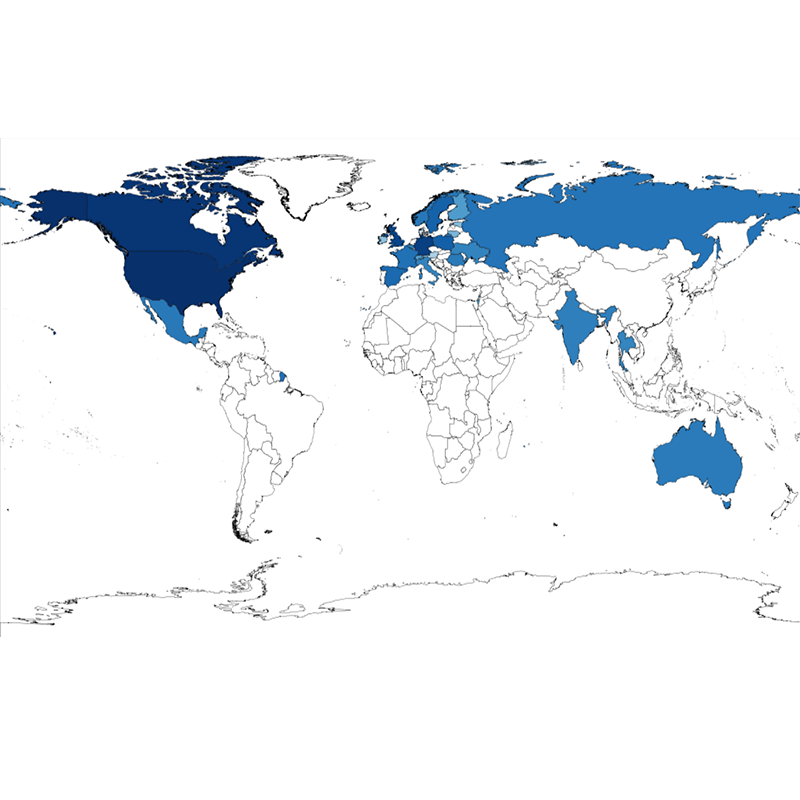
\includegraphics[width=1.1\textwidth]{figures/figure9.png}
                    \caption{SMS地址分布}
                    \label{figure9_WeChat}
                \end{figure}

                \column{.26\textwidth}
                \begin{figure}
                    \centering
                    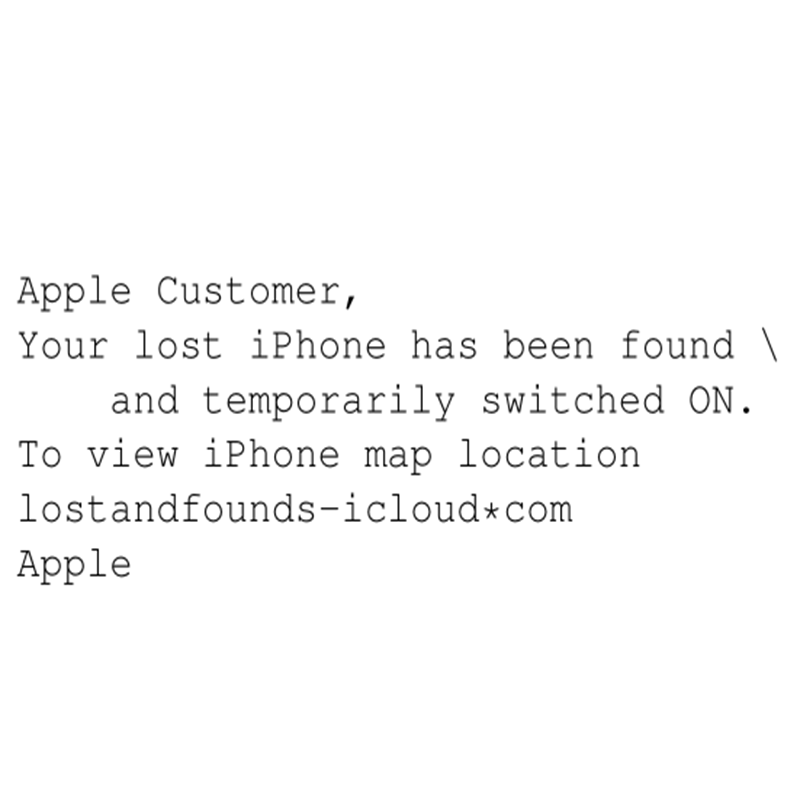
\includegraphics[width=1.1\textwidth]{figures/figure10.png}
                    \caption{钓鱼短信实例}
                    \label{figure10_Talk2}
                \end{figure}

                \column{.26\textwidth}
                \begin{figure}
                    \centering
                    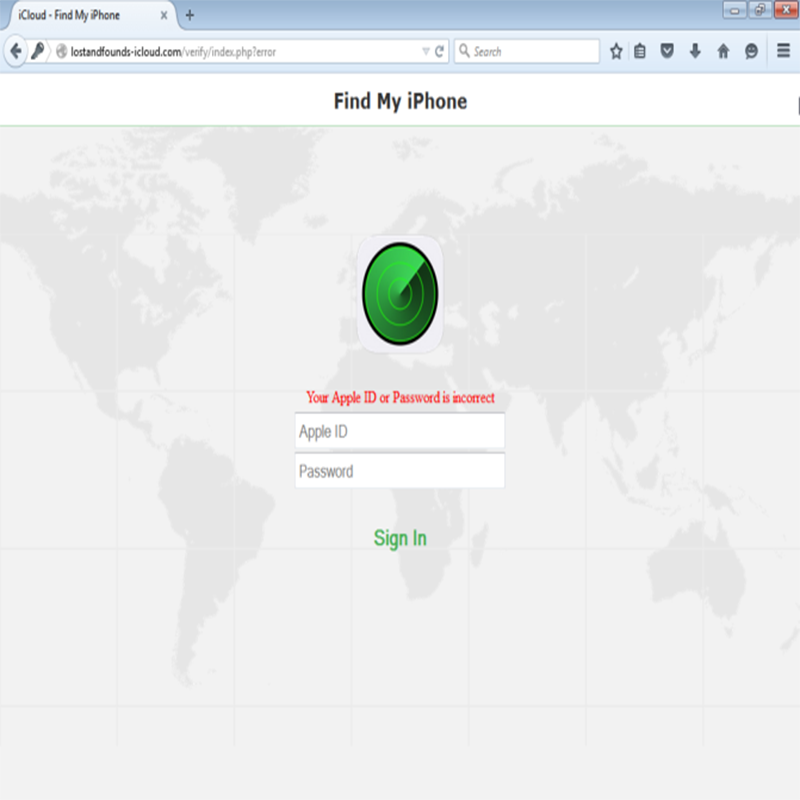
\includegraphics[width=1.1\textwidth]{figures/figure11.png}
                    \caption{钓鱼网站}
                    \label{figure11_Talk2}
                \end{figure}

            \end{columns}

		\end{frame}

\section[结论]{结论}


		\begin{frame}
		  \frametitle{\textbf{结论}}
		
		  \begin{itemize}
		    \item SMS生态系统在智能手机时代出现了新的发展,加入了更多新的设备和参与者。
		    \item 公共网关为用户提供了基于SMS的各种安全解决方案。
            \item 根据该研究,将SMS作为安全信道传递敏感信息存在一定的危险性。一些一次性的消息传递机制亟待改进。
            \item 至于短信滥用,公共网关可以用于规避一些安全性较差的认证机制,或进行PVA欺诈行为。
		  \end{itemize}
		\end{frame}


\section*{}
            \begin{frame}

                \begin{center}
                    \begin{minipage}{1\textwidth}
                        \setbeamercolor{mybox}{fg=white, bg=black!60!green}
                        \begin{beamercolorbox}[wd=0.70\textwidth, rounded=true, shadow=true]{mybox}
                        \LARGE \centering Thanks for Listening.
                        \end{beamercolorbox}
                    \end{minipage}
                \end{center}

                \begin{figure}[!t]
                    \centering
                    
\includegraphics[width=.8\textwidth]{figures/figure5.png}
                    \label{figure4_ad}
                \end{figure}
            \end{frame}

\end{document} 